\pagestyle{empty} % Limpa o cabeçalho e o rodapé
\onehalfspacing % Espaçamento entre-linhas de 1,5
% \hyphenpenalty=10000 % To prevent hyphenation
\pretolerance=10000 % To avoif overful lines
%\selectlanguage{english}
\setcounter{ex}{0} % counter for exercises
\selectlanguage{brazilian}
%\pagenumbering{arabic} % Uncomment this line if you want renumber pages for each chapter
\renewcommand{\chaptername}{Tutorial}
\chapter{TNT - tipos de caracteres e topologias de consenso}\label{tut6}
\rhead{\tiny Instituto de Biociências --USP: BIZ0433 - Inferência Filogenética: Filosofia, Método e Aplicações}
\cfoot{\tiny \cc \ccby \ccsa \href{http://creativecommons.org/licenses/by-sa/4.0/}{Creative Commons Attribution-ShareAlike 4.0 International License}}
%\vspace{5pt}
{\large \sc BIZ0433 - Inferência Filogenética: Filosofia, Método e Aplicações.}\par
%\vspace{10pt}
\par
\minitoc % for table of contents within the chapter
\newpage
\section*{}\addcontentsline{toc}{section}{Objetivo}
\onehalfspacing
\vspace*{5pt}
\begin{center}
\emph{\begin{large}Objetivo\end{large}}\label{tut6:Objetivo}
\vspace{2pt}
\end{center}
%% TEXTO DO RESUMO
O primeiro objetivo deste tutorial é apresentar como caracteres são, ou podem ser tratados em análises filogenéticas. Neste componente do tutorial iremos explorar os impactos do ordenamento de caracteres em inferência filogenética e aplicação de custos arbitrários para séries de transformação. O segundo objetivo deste tutorial é apresentar algumas técnicas de consenso e como computá-las operacionalmente em TNT. Por fim, é apresentado um protocolo para averiguar estabilidade de topologias de consenso em espaços de árvores complexos. Os arquivos associados a este tutorial estão disponíveis em \url{http://lhe.ib.usp.br/cladistica}. Você pode baixá-los diretamente com o seguinte comando:

\begin{center}
\small \texttt{wget http://lhe.ib.usp.br/downloads/tutorial\_06.zip}\\
\end{center}



\newpage
\pagestyle{fancy} % Inclui o cabeçalho definido no meta.tex
%\pagenumbering{arabic} % Números das páginas em arábicos
\begin{refsection}
\renewcommand*{\finalnamedelim}{\addspace\&\space}% Usar '&' ao invés de 'e'.

%%%%%%%%%%%%%%%%%%%%%%%%%%%% HERE TEXT STARTS %%%%%%%%%%%%%%%%%%%%%%%%%%%% 
\section{Tipos de caracteres}\label{tut6:chartypes}

Dentro do contexto de homologia estática de caracteres (\textit{senso} \textcite{Wheeler_2001}), no qual caracteres e seus respectivos estados de caráter (\ie{~} séries de transformação) são postulados a priori, existem 3 classes de caracteres: aditivos (ordenados), não-aditivos (não-ordenados) e caracteres de Sankoff (matrizes de custo). Caracteres aditivos \parencite{Farris_1970} são aqueles em que o custo de transformação é determinado pela diferença entre o índice de cada estado no qual cada índice sucessivo representa um incremento de proposições de homologias mais restritivo \parencite{wheeler_2012}. Considere por exemplo a Figura \ref{tut6:fig:chartypes}A. Assumindo que a raiz desta transformação é o estado ``\texttt{0}'', a aquisição do estado ``\texttt{2}'' assume que a transformação passou pelo estado ``\texttt{1}'', ou seja, ``\texttt{0}'' $\rightarrow$ ``\texttt{1}'' $\rightarrow$ ``\texttt{2}''. Por outro lado, séries de transformações não-aditivas \parencite[][]{Fitch_1971}, o custo de cada transformação é constante entre qualquer par de estados de caráter (veja  Figura \ref{tut6:fig:chartypes}B). Neste caso, a aquisição do estado ``\texttt{2}'' assume apenas uma transformação independente do estado plesiomórfico do qual este derivou (\textit{i.e.}, ``\texttt{0}'', ``\texttt{1}'', ou ``\texttt{3}''; Figura \ref{tut6:fig:chartypes}B).\\

%%%%%%%%%%%%%%%%%%%%%%%%%%% FIGURA CHAR %%%%%%%%%%%%%%%%%%%%%%%%%%%
%  \vspace{-1em}
  \begin{figure}[H]
    %\ffigbox[\FBwidth]
      {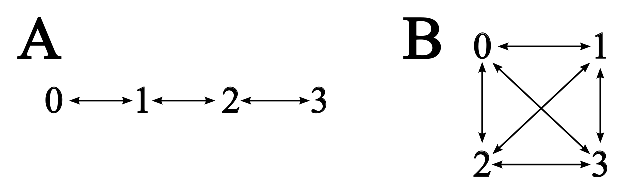
\includegraphics[scale=1.00]{figures/tut6/character_types.eps}}
	{\caption[Tipos de caracteres: aditivo e não-aditivo]{Tipos de caracteres: aditivo e não-aditivo. \textbf{A}, caráter aditivo; \textbf{B}, caráter não-aditivo.}\label{tut6:fig:chartypes}}
  \end{figure}

%%%%%%%%%%%%%%%%%%%%%%%%%%% FIM DA FIGURA CHAR %%%%%%%%%%%%%%%%%%%%%

Não há consenso na literatura sobre ordenar ou não séries de transformações de caracteres multi-estados (seja \parencite{Hauser_and_Presch_1991, Slowinski_1993, Nixon_and_Carpenter_2011}). \textcite[][:8]{Nixon_and_Carpenter_2011} argumenta: 

\begin{quotation}
\textit{Additive characters are just more explicit, compound hypotheses of homology. The fact that nonadditive codings tend to produce shorter trees does not a priori make them better. Throwing away characters, or lying, can also produce shorter trees. Nonadditive codings are better only when they are better justified (or more defensible) in terms of homology assessment. In fact, a nonadditive multistate character implies ambiguity in our understanding of the homology among the states, because it is not generally possible that all allowed transformations are simultaneously true.}
\end{quotation}

Os argumentos apresentados por \textcite{Nixon_and_Carpenter_2011} sugerem que é necessário explicitar os critérios que levam o investigador a considerar determinada série de transformação de forma aditiva. Isso porque seguindo o raciocínio desses autores, o ordenamento revela maior conhecimento sobre as noções de homologia putativa entre os estados. No entanto, \textcite{Hauser_and_Presch_1991} verificaram que a grande maioria dos estudos que consideravam séries de transformações ordenadas não apresentava nenhum critério para determinar a ordem dos estados de caracteres. Tendências morfológicas, sequências ontogenéticas (raramente disponíveis), similaridade entre estados, entre outros, podem ser utilizadas para justificar ordem de estados de caráter \parencite[mas veja][]{Hauser_and_Presch_1991} --, nenhuma delas sem assumir premissas cuja necessidade fica a cargo do pesquisador. Considere que o ordenamento de estados de caráter representa uma hipótese específica sobre a relação evolutiva entre os estados de caráter. 

	Vejamos como o TNT permite implementar estes conceitos. A definição de tipos de caracteres em TNT é feita pelo comando ``\texttt{ccode}'':
\\
\texttt{tnt*>help ccode}\\
\texttt{CCODE}\\
\texttt{\indent !  re-sets ccode to the one defined in the data file }\\
\texttt{\indent Other than that, sets character codes.  Specifiers are: }\\
\texttt{\indent\indent +~~~make following character(s) additive }\\
\texttt{\indent\indent -~~~~~"~~~~~~"~~~~~~~~~"~~~~~~~~non-additive }\\
\texttt{\indent\indent [~~~~~"~~~~~~"~~~~~~~~~"~~~~~~~~active }\\
\texttt{\indent\indent ]~~~~~"~~~~~~"~~~~~~~~~"~~~~~~~~inactive }\\
\texttt{\indent\indent (~~~~~"~~~~~~"~~~~~~~~~"~~~~~~~~Sankoff }\\
\texttt{\indent\indent )~~~~~"~~~~~~"~~~~~~~~~"~~~~~~~~non-Sankoff }\\
\texttt{\indent\indent /N~~~apply weight N to following character(s) }\\
\texttt{\indent\indent =N~~~apply N additional steps to following character(s) }\\

Vejamos como podemos implementar caracteres aditivos e não aditivos em TNT. Considere a seguinte matrix:
\\
\texttt{xread}\\
\texttt{7 6}\\
\texttt{taxon\_A 0000000}\\
\texttt{taxon\_B 1000000}\\
\texttt{taxon\_C 2000011}\\
\texttt{taxon\_D 3001112}\\
\texttt{taxon\_E 4111212}\\
\texttt{taxon\_F 5111322}\\
\texttt{;}\\

Considere os seguintes comandos e seus respectivos efeitos:

\begin {myindentpar}{0.3cm}
\begin{enumerate}[\itshape i.]
	\item{``\texttt{ccode + 0}''}: Faz com que TNT considere o caráter \texttt{0} additivo.\\
	\item{``\texttt{cc + 0 4.6}''}: Faz com que TNT considere os caracteres \texttt{0, 4, 5} e \texttt{6} aditivos\footnote{Você pode abreviar esse comando utilizando simplesmente ``\texttt{cc}''}.\\
	\item{``\texttt{cc -.}''}: Faz com que TNT considere todos caracteres não-aditivos.\\
	\item{``\texttt{cc}''}: Faz com que TNT exiba a codificação de cada caráter, por exemplo:\\
\texttt{Ccode~~}\\
\texttt{~~~+[/1~~0~~~~~-[/1~~1~~~~~-[/1~~2~~~~~-[/1~~3~~~~~+[/1~~4~~~~~}\\
\texttt{~~~+[/1~~5~~~~~+[/1~~6~~~~~;}\\

Neste exemplo acima, os caracteres \texttt{0, 4, 5} e \texttt{6} serão considerados aditivos (\textit{i.e.}, identificados pelo símbolo ``\texttt{+}''). Observe também que a notação ``\texttt{[/1}'', comum a todos os caracteres, indica que todos os caracteres estão sendo considerados e possuem peso \texttt{1}.\\

\end{enumerate}
\end{myindentpar}


\stepcounter{ex}
\begin{blackBlock}{\textbf{Exercicio 6.\arabic{ex}}}\label{tut6:ex:6.1}

Neste exercício, iremos utilizar a matriz contida no arquivo \texttt{exemplo\_1a.tnt} para implementar os conceitos descritos acima.

\end{blackBlock}


\begin {myindentpar}{0.5cm}
\begin{enumerate}[\itshape i.]
	\item{Faça uma análise cladística da matrix em TNT do arquivo \texttt{exemplo\_1a.tnt} e responda:}
		\begin {myindentpar}{0.5cm}
		\begin{enumerate}[\itshape a.]
		\item{A topologia depende do ordenamento de algum caráter? Justifique.}
\\
\\
\\
\\
\\
\\
		\line(1,0){400}\\
		\line(1,0){400}\\
		\line(1,0){400}\\

		\end{enumerate}
		\end{myindentpar}

	\item{Faça uma análise cladística da matriz em TNT do arquivo \texttt{exemplo\_1b.tnt} e responda:}
		\begin {myindentpar}{0.5cm}
		\begin{enumerate}[\itshape a.]
		\item{Qual caráter quando considerado aditivo reduz o número de topologias igualmente parcimoniosa?}
		\line(1,0){400}\\

		\item{Existe algum caráter cujo ordenamento  (\textit{i.e.}, ``\texttt{0}'' $\rightarrow$ ``\texttt{1}'' $\rightarrow$ ``\texttt{2}'' ...)  pode ser defendido utilizando o critério de parcimônia? Justifique.}
\\
\\
\\
\\
\\
\\
		\line(1,0){400}\\
		\line(1,0){400}\\
		\line(1,0){400}\\
		\item{Supondo que você tenha uma justificativa para ordenar o caráter que reduz o número de topologias, implemente a ordenação deste caráter e salve no arquivo \texttt{exemplo\_1b\_recons.txt} a reconstrução do caráter 2\footnote{numeração de acordo com TNT. Veja Tutorial 5 item \ref{tut5:recons} para detalhes de como verificar reconstruções em TNT.} e responda: Quantas reconstruções o TNT postula para esse caráter?}

		\line(1,0){400}\\

		\end{enumerate}
		\end{myindentpar}
\end{enumerate}
\end{myindentpar}

O ordenamento de caracteres não precisa ser necessariamente linear (\textit{i.e.}, ``\texttt{0}'' $\rightarrow$ ``\texttt{1}'' $\rightarrow$ ``\texttt{2}'' $\rightarrow$ ``\texttt{3}'' $\rightarrow$ ``\texttt{4}'') como nos exemplos acima. Considere, por exemplo, a Figura \ref{tut6:fig:chartypes_matrix}. Nela, as relações entre os estados de caráter \texttt{0--4} é apresentada de forma ramificada. Assumir essa estrutura hierárquica entre os estados de caráter não é diferente do ordenamento linear desta série de transformação. No entanto, esta relação entre os estados requer uma implementação distinta em TNT. A matriz à direita na Figura \ref{tut6:fig:chartypes_matrix} expressa os custos associados entre cada uma das transformações possíveis. Por exemplo, a transformação ``\texttt{1}'' $\rightarrow$ ``\texttt{3}'' tem o custo de 3 transformações (\textit{i.e.}, ``\texttt{1}'' $\rightarrow$ ``\texttt{0}'' $\rightarrow$ ``\texttt{2}'' $\rightarrow$ ``\texttt{3}'').


%%%%%%%%%%%%%%%%%%%%%%%%%%% FIGURA CHAR %%%%%%%%%%%%%%%%%%%%%%%%%%%
%  \vspace{-1em}
  \begin{figure}[H]
    %\ffigbox[\FBwidth]
      {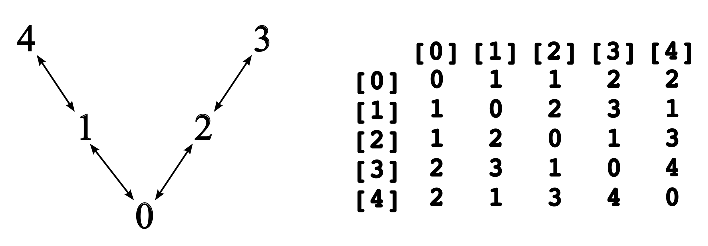
\includegraphics[scale=1.00]{figures/tut6/character_types_matrix.eps}}
	{\caption[Tipos de caracteres: matriz de transformção]{Tipos de caracteres: matriz de transformção.}\label{tut6:fig:chartypes_matrix}}
  \end{figure}

%%%%%%%%%%%%%%%%%%%%%%%%%%% FIM DA FIGURA CHAR %%%%%%%%%%%%%%%%%%%%%

Esta matriz define os custos de transformação do que chamamos caracteres de Sankoff \parencite{Sankoff_1975}. Matrizes de Sankoff são implementadas para caracteres para os quais assume-se custos arbitrários de transformação, via de regra associados à uma ou mais premissas sobre a evolução destes caracteres. Embora \textcite{Sankoff_1975} tivesse desenvolvido este procedimento de otimização para estudar evolução macromolecular, matrizes de Sankoff podem ser aplicadas a qualquer série de transformação -- mesmo binária.

	Em TNT, a implementação de matrizes de Sankoff requer os seguintes passos:
\begin {myindentpar}{0.3cm}
\begin{enumerate}[\itshape 1.]
	\item{Definição da matriz de Sankoff:}\\
	A definição de matrizes de Sabkoff é feita pelo comando \texttt{smatrix} do TNT obedecendo a seguinte sintaxe:\\
\texttt{smatrix =S (xxxx) ...costs... ;}\\
onde ``\texttt{S}'' é um número entre 0-31 e indexa internamente a matriz no TNT; ``\texttt{xxxx}'' é o nome atribuído à matriz (opcional) e ``\texttt{costs}'' são os custos de cada transformação. Os custos são definidos considerando a direção da transformação, como por exemplo \texttt{0>4 2} que atribui custo 2 para a transformação ``\texttt{0}'' $\rightarrow$ ``\texttt{4}'', ou estabelecendo custos simétricos, como por exemplo \texttt{0/2  1} que atribui custo 1 para as transformações ``\texttt{0}'' $\rightarrow$ ``\texttt{2}'' ou ``\texttt{2}'' $\rightarrow$ ``\texttt{0}''. 

	\item{Aplicação da matriz de Sankoff:}\\
	Uma vez definida a matriz de Sankoff, ela deve ser aplicada ao caráter desejado, ou caracteres utilizando o comando ``\texttt{smatrix +S N}'' ou ``\texttt{smatrix +xxxx N}'', onde ``\texttt{N}'' é o caráter para o qual se quer aplicar a matriz de Sankoff.

	\item{Implementação matriz de Sankoff em \texttt{ccode}:}\\	
	Finalmente, é necessário habilitar o caráter de Sankoff no TNT utilizando o comando ``\texttt{ccode (N''}.

\end{enumerate}
\end{myindentpar}


\stepcounter{ex}
\begin{blackBlock}{\textbf{Exercicio 6.\arabic{ex}}}\label{tut6:ex:6.1}

Neste exercício, você deverá criar uma matriz de Sankoff e implementar esta função de custo na análise filogenética usando TNT. \textbf{No entanto, antes de executar esse exercício examine as últimas linhas do arquivo \texttt{exemplo\_2.tnt}.}

\end{blackBlock}

\begin {myindentpar}{0.5cm}
\begin{enumerate}[\itshape i.]
	\item{Construa uma matriz te Sankoff para a série de transformação ordenada ilustrada na Figura \ref{tut6:fig:chartypes_matrix_ex}.}\\
%%%%%%%%%%%%%%%%%%%%%%%%%%% FIGURA CHAR %%%%%%%%%%%%%%%%%%%%%%%%%%%
%  \vspace{-1em}
  \begin{figure}[H]
    %\ffigbox[\FBwidth]
      {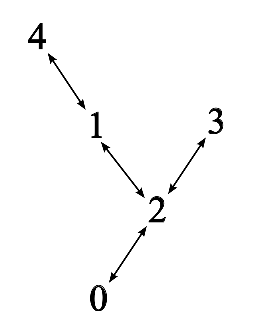
\includegraphics[scale=1.00]{figures/tut6/character_types_ex2.eps}}
	{\caption[Matriz de Sankoff: Exercício \ref{tut6:newtech:ex2}]{Série de transformação ordenada não-linear.}\label{tut6:fig:chartypes_matrix_ex}}
  \end{figure}

%%%%%%%%%%%%%%%%%%%%%%%%%%% FIM DA FIGURA CHAR %%%%%%%%%%%%%%%%%%%%%

\begin{table}[h]
\begin{tabular}{|c|c|c|c|c|c|}\hline
 & $[$\texttt{0}$]$ & $[$\texttt{1}$]$ & $[$\texttt{2}$]$ & $[$\texttt{3}$]$ & $[$\texttt{4}$]$ \\\hline
$[$\texttt{0}$]$ & - &  &  &  &  \\\hline
$[$\texttt{1}$]$ &  & - &  &  &  \\\hline
$[$\texttt{2}$]$ &  &  & - &  &  \\\hline
$[$\texttt{3}$]$ &  &  &  & - &  \\\hline
$[$\texttt{4}$]$ &  &  &  &  & - \\\hline
\end{tabular}
\end{table}


	\item{Com base na sua matriz de Sankoff, defina a \texttt{smatrix} abaixo:}\\
\texttt{smatrix =0 (minha\_matriz) ... }

\vspace{90pt}

	\item{Execute uma busca no TNT com o arquivo \texttt{exemplo\_2.tnt} e responda:}\\
	A implementação da matriz de Sankoff teve algum impacto na reconstrução do caráter 2? Justifique.
	
	\line(1,0){400}\\
	\line(1,0){400}\\
	\line(1,0){400}\\

\end{enumerate}
\end{myindentpar}

Matrizes de Sankoff são muito utilizadas em análise de dados moleculares -- em concordância com sua concepção inicial \parencite{Sankoff_1975}. A Figura \ref{tut6:fig:tv_ts} representa duas classes de transformações (\textit{i.e.}, transições e transversões) de caracteres genotípicos -- sequências nucleotídicas -- comumente utilizadas em análises filogenéticas de dados moleculares. A premissa associada ao custo diferencial entre essas duas classes de transformações reside na expectativa de que transversões (\textit{i.e.}, purinas $\longleftrightarrow$ pirimidinas) tem impacto bioquímico mais acentuado nas moléculas e, consequentemente, estão sob maiores restrições de transformação do que transições (\textit{i.e.}, purinas $\longleftrightarrow$ purinas ou pirimidinas $\longleftrightarrow$ pirimidinas). Sequências nucleotídicas são sempre consideradas caracteres não-aditivos e via de regra são submetidos à matrizes de Sankoff.

%%%%%%%%%%%%%%%%%%%%%%%%%%% FIGURA CHAR %%%%%%%%%%%%%%%%%%%%%%%%%%%
%  \vspace{-1em}
  \begin{figure}[H]
    %\ffigbox[\FBwidth]
      {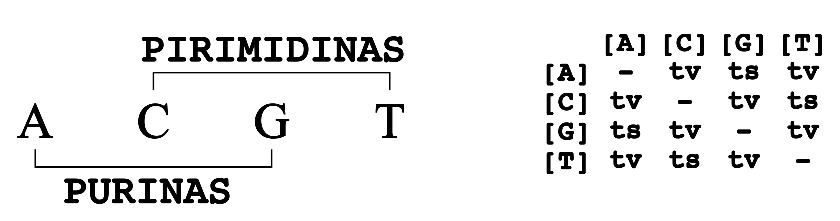
\includegraphics[scale=1.00]{figures/tut6/tv_ts.eps}}
	{\caption[Classes de transformação de caracteres genotípicos]{Classes de transformação de caracteres genotípicos: transições e transversões}\label{tut6:fig:tv_ts}}
  \end{figure}

%%%%%%%%%%%%%%%%%%%%%%%%%%% FIM DA FIGURA CHAR %%%%%%%%%%%%%%%%%%%%%

\stepcounter{ex}
\begin{blackBlock}{\textbf{Exercício 6.\arabic{ex}}}\label{tut6:ex:6.3}

Considere os dados na matriz do arquivo \texttt{exemplo\_3.tnt} e execute as seguintes tarefas:

\end{blackBlock}

\begin {myindentpar}{0.5cm}
\begin{enumerate}[\itshape i.]
	\item{Faça uma análise filogenética destes dados e responda:}\\
		\begin {myindentpar}{0.5cm}
		\begin{enumerate}[\itshape a.]
		  \item{Qual é a topologia recuperada e qual é o seu custo (\textit{i.e.}, número de transformações)?}
\vspace{100pt}

		\line(1,0){400}\\
		\end{enumerate}
		\end{myindentpar}
	\item{Abaixo defina a matriz de Sankoff no qual você atribuirá peso 2 para transversões e peso 1 para transições:}\\
\texttt{smatrix =0  C/A \_ G/A \_ G/C \_ T/A \_ T/C \_ T/G \_;}\\

	\item{Modifique o arquivo \texttt{exemplo\_3.tnt} de modo que todos os caracteres sejam analisados de acordo com sua matriz de Sankoff, reanalise esses dados e responda:}\\
		\begin {myindentpar}{0.5cm}
		\begin{enumerate}[\itshape a.]
		  \item{A implementação desta nova função de custo modificou seus resultados? Explique.}
		  \\
		  \\
		  \\
		  \\
		\line(1,0){400}\\
		\line(1,0){400}\\
		\line(1,0){400}\\
		\line(1,0){400}\\

		\end{enumerate}
		\end{myindentpar}

\end{enumerate}
\end{myindentpar}

\section{Árvores de consenso}\label{tut6:consenso}

Métodos de consenso apresentam um sumário de informações contidas em um conjunto de topologias. Fundamentalmente, topologias de consenso é o resultado da aplicação de uma série de regras e/ou algoritmos sob um conjunto de topologias que resulta em uma única árvore com o mesmo conjunto de terminais \parencite{Bryant_2003}. De acordo com \textcite{Bryant_2003}, há uma série de controvérsias relacionadas à topologias de consenso; no entanto estas estão mais relacionadas com as interpretações sobre as topologias de consenso do que com os métodos usados para gerá-las \parencite[veja,][]{Barrett_et_al_1991}.

Há algumas generalidade sobre topologias de consenso que devem ser consideradas. A primeira delas é que topologias de consenso são sumários de informação e o número de transformações nestas topologias é via de regra subótima \parencite{Miyamoto_1985, Carpenter_1988} -- portanto, \textbf{otimizações em topologias de consenso não devem ser consideradas}. Outra propriedade comum à topologias de consenso, especialmente relacionadas com o sumário de informações filogenéticas provenientes de fontes de dados distintas, é que em alguns casos a topologia de consenso difere do resultado que seria obtido considerando a análise simultânea destas bases de dados (seja \textcite{Barrett_et_al_1991}). Portanto, considere que a maioria das técnicas de consenso foram concebidas como ferramentas de representação e não para \textbf{inferência filogenética} propriamente dita (mas veja \textcite{Holder_et_al_2008}).
	
Neste componente do tutorial iremos explorar três tipos de consenso, aqueles mais frequentemente utilizados em análises filogenéticas. Essa exposição breve sobre o tópico tem mais caráter operacional do que fomentar as discussões sobre o uso de métodos de consenso em inferência filogenética.

\subsection{Consenso estrito}\label{tut6:consenso:strict}

O consenso estrito \parencite{Rohlf_1982}, como o nome sugere, é o mais simples -- e o mais frequente na literatura. Esta técnica de consenso produz uma topologia que é o sumário de todos os componentes (\textit{i.e.}, clados) que estão presentes em \textbf{todas} as topologias fundamentais.

\subsection{Consenso semi-estrito}\label{tut6:consenso:semi_strict}

O consenso semi-estrito \parencite{Bremer_1990}, também conhecido como \textit{compatible components}, é menos restritivo do que o consenso estrito. Neste método de consenso a topologia final contém todos os componentes presentes nas topologias fundamentais \textbf{com a inclusão daqueles que não são contraditórios entre si}. Colocado de outra forma, enquanto que no cálculo do consenso estrito um determinado componente só será representado se estiver necessariamente em todas as topologias fundamentais, no consenso semi-estrito ele deve estar presente em pelo menos uma delas e não ser contradito por nenhum outro componente das demais topologias que fazem parte do conjunto.

\subsection{Consenso de Maioria}\label{tut6:consenso:majority}

O consenso de maioria (\textit{i.e.}, \textit{majority-rule}; \textcite{Margush_and_McMorris_1981}) baseia-se na frequência dos clados presentes nas topologias fundamentais. \textcite{Margush_and_McMorris_1981} define este tipo de consenso como sendo topologias de consenso M\textsubscript{\textit{l}} no qual o parâmetro \textit{l} define a porcentagem mínima da frequência dos componentes que deverão estar presentes na topologia de consenso. Observe que se \textit{l} é 100\% você obtém o consenso estrito das topologias fundamentais. Este tipo de consenso é utilizado em análises de suporte e de inferência filogenética que utiliza como critério de otimização probabilidades posteriores \parencite[\textit{i.e.}, análises bayesianas; veja][]{Holder_et_al_2008}.\\


\stepcounter{ex}
\begin{blackBlock}{\textbf{Exercício 6.\arabic{ex}}}\label{tut6:ex:6.4}

Neste exercício iremos explorar as propriedades destes métodos de consenso utilizando as topologias existentes no arquivo \texttt{exemplo\_4.tnt}.

\end{blackBlock}


\begin {myindentpar}{0.3cm}
\begin{enumerate}[\itshape i.]
	\item{Verifique os clados em cada uma das três topologias.}
	\item{Calcule o consenso estrito utilizando o comando ``\texttt{ne}''.}
	\item{Represente a tolologia de consenso no espaço abaixo e compare novamente com as topologias fundamentais.}

\vspace{100pt}

	\item{Calcule o consenso semi-estrito utilizando o comando ``\texttt{comcomp}''.}
	\item{Represente a topologia de consenso no espaço abaixo e compare novamente com as topologias fundamentais.}

\vspace{100pt}

	\item{Como é a resolução desta topologia de consenso em relação à topologias fundamentais?}

	\line(1,0){400}\\
	\line(1,0){400}\\

	\item{Calcule o consenso de maioria utilizando o comando ``\texttt{majority = 50}''.}
	\item{Represente a topologia no espaço abaixo e compare novamente com as topologias fundamentais.}

\vspace{100pt}

	\item{Qual observação você faria ao comparar as topologias fundamentais com a de consenso de maioria?}

	\line(1,0){400}\\
	\line(1,0){400}\\


\end{enumerate}
\end{myindentpar}


\subsection{Estabilidade do consenso}\label{tut6:consenso:stability}

Independente da técnica de consenso que você deseja utilizar para calcular topologias de consenso, é importante que você tenha uma boa amostra de topologias do seu espaço de árvore -- principalmente quando este apresenta relativa complexidade. Neste último componente sobre o assunto irei sugerir um protocolo para verificar se, potencialmente, você obteve estabilidade em sua topologia de consenso. Considere que nem sempre a inspeção visual é uma forma imediata de observar se houve ou não mudança entre uma topologia de consenso e outra à medida em que você compila topologias com o mesmo custo. Considere por exemplo os arquivos \texttt{consenso\_*.tre}. Suponha que esses arquivos foram obtidos com buscas incrementalmente mais agressivas e que à cada uma delas um número maior de topologias foi amostrado. Se você listar de forma longa esses arquivos (\textit{i.e.}, com o comando \texttt{ls -l}), você obterá:\\

\noindent\texttt{-rw-rw-r--~1~alan~alan~84~Apr~~7~20:29~consenso\_1.tre}\\
\texttt{-rw-rw-r--~1~alan~alan~82~Apr~~7~20:33~consenso\_2.tre}\\
\texttt{-rw-rw-r--~1~alan~alan~80~Apr~~7~20:33~consenso\_3.tre}\\
\texttt{-rw-rw-r--~1~alan~alan~80~Apr~~7~20:33~consenso\_4.tre}\\

A primeira dica refere-se ao tamanho desses arquivos. Observe que o arquivo consenso\_1.tre possui 84 bites, o consenso\_2.tre 82 e os demais 80. O número decremental de bites sugere que os arquivos possuem um número menor de caracteres, ou seja, parênteses que são usados para definir grupos! Inspecione o conteúdo destes arquivos.

No caso da sugestão acima, você deve considerar que dois arquivos podem possuir o mesmo número de bites e, no entanto, suas topologias podem ser distintas. Um outra forma de verificar, ou comparar essas topologias de forma mais segura, é utilizar o comando ``\texttt{diff}'' -- um comando interno de LINUX/UNIX. Se você executar em um terminal:\\

\shellcmd{diff -q -s consenso\_1.tre consenso\_2.tre}\\

você deverá obter:

\texttt{Files consenso\_1.tre and consenso\_2.tre differ}\\

Por outro lado, se você executar em um terminal:

\shellcmd{diff -q -s consenso\_3.tre consenso\_4.tre}\\

você deverá obter:

\texttt{Files consenso\_3.tre and consenso\_4.tre are identical}\\

\stepcounter{ex}
\begin{blackBlock}{\textbf{Exercicio 6.\arabic{ex}}}\label{tut6:ex:6.4}

Neste exercício você irá explorar estabilidade de consensos. Você deverá fazer algumas análises em TNT, compilar os dados na Tabela \ref{tut6:table:stability} e identificar a partir de que momento destas análises você obteve a estabilidade de sua topologia de consenso.

\end{blackBlock}

	Considere os seguintes comandos de TNT e suas respectivas ações:\\
\texttt{log log\_run.txt;}\\
\texttt{xmu: hold 10 rep 50 ratchet 5 drift 5 fuse 10;}\\
\texttt{xmu;}\\
\texttt{ne*;}\\
\texttt{tchoose/;}\\
\texttt{tsave* busca\_1.tre;}\\
\texttt{save;}\\
\texttt{tsave/;}\\
\texttt{log/;}\\

Esta sequência de comandos abre um arquivo de \textit{log} chamado \texttt{log\_run.txt}, executa uma busca usando novas tecnologias em TNT para um determinado arquivo de entrada, calcula o consenso estrito e faz com que a topologia de consenso seja inserida no \textit{buffer} de memória do TNT, seleciona a última topologia e descarta as demais (no caso a topologia de consenso é mantida), abre um arquivo para salvar topologias chamado \texttt{busca\_1.tre}, salva a topologia e fecha os arquivos de árvore e de \textit{log}.\\

Neste exercício você deverá estabilizar o consenso as topologias encontradas na matriz \texttt{zilla.tnt} em 10 buscas. Os números de topologias encontradas em cada uma dessas análises deverá ser sempre superior à encontrada na análise anterior. Você deverá preencher a tabela abaixo (Tabela \ref{tut6:table:stability}) e comparar os arquivos que julgar necessário com o comando \texttt{diff -q -s [arquivo1] [arquivo2]}.
	
%%%%%%%%%%%%%%%%%%%%%%%%%%% TABELA DE CONSENSO %%%%%%%%%%%%%%%%%%%%%%%%%%% 
%\begin{landscape}
\pagestyle{fancy}
\begin{center}

\begin{longtable}{|c|c|c|c|c|c|c|}
\caption[Tabela \ref{tut6:table:stability}: Buscas heurísticas e estabilidade de consenso em TNT]{Buscas heurísticas e estabilidade de consenso em TNT} \label{tut6:table:stability} \\


\hline\hline \textbf{Busca} & \textbf{Parâmetros de Busca}  & \textbf{\# Topologias retidas} & \textbf{Tamanho do Arquivo}\\
\endfirsthead

\multicolumn{6}{c}{{\bfseries \tablename\ \thetable{} -- Continuação.}}\\
\hline\hline \textbf{Busca} & \textbf{Parâmetros de Busca}  & \textbf{\# Topologias retidas} & \textbf{Tamanho do Arquivo}\\
\endhead
%\hline \multicolumn{6}{r}{{--continua na próxima página}} \\ \hline
%\endfoot
\hline \hline
%\hline \multicolumn{6}{l}{Consulte a página \url{http://wiki.linuxquestions.org/wiki/Linux_software_equivalent_to_Windows_software}.}
\endlastfoot

\hline1 &  &  & \\
\hline2 &  &  & \\
\hline3 &  &  & \\
\hline4 &  &  & \\
\hline5 &  &  & \\
\hline6 &  &  & \\
\hline7 &  &  & \\
\hline8 &  &  & \\
\hline9 &  &  & \\
\hline10 &  &  & \\

\end{longtable}
\end{center}
%\end{landscape}

%%%%%%%%%%%%%%%%%%%%%%%%%%% FIM DA TABELA CONSENSO %%%%%%%%%%%%%%%%%%%%%%%%%%
	
Observações de comparação:\\
	\line(1,0){400}\\
	\line(1,0){400}\\
	\line(1,0){400}\\
	\line(1,0){400}\\

%%%%%%%%%%%%%%%%%%%%%%%%%%%% HERE ENDS TEXT AND ADDS REFERENCES %%%%%%%%%%%%%%%%%%%%%%%%%%%% 
\section{Referências}\label{tut6:refs}
\printbibliography[heading=none]
\end{refsection}
%

